%% This is file `elsarticle-template-1-num.tex',
%% %% Copyright 2009 Elsevier Ltd
%%
%% This file is part of the 'Elsarticle Bundle'.
%% ---------------------------------------------
%%
%% It may be distributed under the conditions of the LaTeX Project Public
%% License, either version 1.2 of this license or (at your option) any
%% later version.  The latest version of this license is in
%%    http://www.latex-project.org/lppl.txt
%% and version 1.2 or later is part of all distributions of LaTeX
%% version 1999/12/01 or later.
%%
%% The list of all files belonging to the 'Elsarticle Bundle' is
%% given in the file `manifest.txt'.
%%
%% Template article for Elsevier's document class `elsarticle'
%% with numbered style bibliographic references
%%
%% $Id: elsarticle-template-1-num.tex 149 2009-10-08 05:01:15Z rishi $
%% $URL: http://lenova.river-valley.com/svn/elsbst/trunk/elsarticle-template-1-num.tex $
%%

\documentclass[preprint,5p,times,twocolumn]{elsarticle}
%\documentclass[final,5p,times,twocolumn]{elsarticle}

%% Use the option review to obtain double line spacing
%% \documentclass[preprint,review,12pt]{elsarticle}

%% Use the options 1p,twocolumn; 3p; 3p,twocolumn; 5p; or 5p,twocolumn
%% for a journal layout:
%% \documentclass[final,1p,times]{elsarticle}
%% \documentclass[final,1p,times,twocolumn]{elsarticle}
%% \documentclass[final,3p,times]{elsarticle}
%% \documentclass[final,3p,times,twocolumn]{elsarticle}
%% \documentclass[final,5p,times]{elsarticle}
%% \documentclass[final,5p,times,twocolumn]{elsarticle}

%% if you use PostScript figures in your article
%% use the graphics package for simple commands
%% \usepackage{graphics}
%% or use the graphicx package for more complicated commands
%% \usepackage{graphicx}
%% or use the epsfig package if you prefer to use the old commands
%% \usepackage{epsfig}

%% The amssymb package provides various useful mathematical symbols
\usepackage{amssymb}
\usepackage{lipsum}
\usepackage{tikz}
\usetikzlibrary{shapes, arrows}


%% Styles for proximity flow chart
\tikzstyle{ccell} = [rectangle, draw, fill=red!20, minimum width=3em, text centered, minimum height=3em]
\tikzstyle{dcell} = [rectangle, draw, fill=brown!20, minimum width=3em, text centered, minimum height=3em]
\tikzstyle{gcell} = [rectangle, draw, fill=yellow!20, minimum width=3em, text centered, minimum height=3em]
\tikzstyle{fcell} = [rectangle, draw, fill=green!20, minimum width=3em, text centered, minimum height=3em]
\tikzstyle{ucell} = [rectangle, draw, fill=white!20, minimum width=3em, text centered, minimum height=3em]
\tikzstyle{line} = [draw, -latex']


\journal{University of Guelph; CIS*4780}

\newcommand{\cond}[3]{P_{#3}(#1|\,#2)$}

\begin{document}

\begin{frontmatter}

\title{Two Dimensional Intelligent Character Recognition; A Rope Of Sand}

%% use optional labels to link authors explicitly to addresses:
%% \author[label1,label2]{<author name>}
%% \address[label1]{<address>}
%% \address[label2]{<address>}

\author[ryan,doug,oliver]{Ryan Pattison, Douglas Anderson, and Oliver Cook}

\address[ryan]{ryan.m.pattison@gmail.com}
\address[doug]{dander01@uoguelph.ca}
\address[oliver]{cooko@uoguelph.ca}


\begin{abstract}

For quite some time computer vision has been used to extract characters from
images in order to gain knowledge from text. In recent years many of the
techniques for recognizing characters has been based on machine learning.

\end{abstract}

\begin{keyword}
%% keywords here, in the form: keyword \sep keyword
Machine Learning \sep
Data Mining \sep
Computer Vision \sep
Intelligent Character Recognition

%% MSC codes here, in the form: \MSC code \sep code
%% or \MSC[2008] code \sep code (2000 is the default)

\end{keyword}

\end{frontmatter}

%%
%% Start line numbering here if you want
%%
%%\linenumbers

%% main text
\section{Introduction}
\label{intro}
\lipsum[1-2]


\section{Process}
\label{process}

\subsection{Overview}
\label{process:overview}
\lipsum[1-3]

\subsection{Feature-Based Approach}
\label{process:featurebased}
\lipsum[1-2]

\subsection{Gold Comparison Approach}
\label{process:gold}
\lipsum{1-3}

\subsection{Proximity Approach}
\label{process:proximity}

Summary of approach paragrah. When it's done this is gonna be flowing elegant
and complete but for now... pfffft %TODO

\begin{figure}[h]
\begin{center}
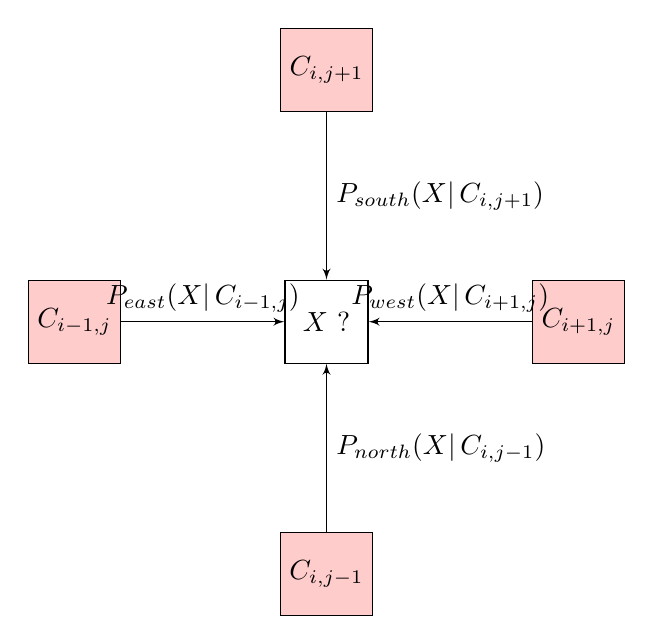
\begin{tikzpicture}[node distance = 3.2 cm, auto]
    \node[ccell](top){$C_{i,j+1}$};
    \node[ucell, below of=top](center){$X$~?};
    \node[ccell, left of=center](left){$C_{i-1,j}$};
    \node[ccell, right of=center](right){$C_{i+1,j}$};
    \node[ccell, below of=center](bottom){$C_{i,j-1}$};

    \path[line] (top)   -- node[right] {$P_{south}(X | \, C_{i,j+1})$} (center);

    \path[line] (left)  -- node[above] {$P_{east}(X | \, C_{i-1,j})$} (center);
    \path[line] (right) -- node[above] {$P_{west}(X | \, C_{i+1,j})$} (center);
    \path[line] (bottom) -- node[right] {$P_{north}(X | \, C_{i,j-1})$} (center);
\end{tikzpicture}
\end{center}
\caption{This figure describes the probability of class $X$ neighbouring cells $C_{i,j}$}
\end{figure}

Let $V_{d}$ be a vector of probabilities, where $n$ is the number of classes,
$d$ is a direction.

\[
\begin{array}{l}
V = P(X),\quad P(X \in C_i) = V_i \\
V = P(X|\,N\!=\!g,\,S\!=\!g,\,E\!=\!d,\,W\!=\!d)  \\
= P(X|\,N\!=\!g)P(X|\,S\!=\!g)P(X|\,E\!=\!d)P(X|\,W\!=\!d) \\
\end{array}
\]

\begin{equation}
V_{d} = \left(P_{d}{(X_{1} | \, C_{d})}, P_{d}{(X_{2} | \, C_{d}),\; \ldots \; , P_{d}{(X_{n} | \, C_{d}})}\right)
\end{equation}

To determine the probability of a cell belonging in a particular class, we assume independence
so that we can multiply the vectors of all directions together using the element-wise product.

\begin{equation}
C_{centre} = V_{north} \circ V_{east} \circ V_{south} \circ V_{west}
\end{equation}

This new vector $C_{centre}$ contains $n$ probabilities that this cell should be
classified as a particular class. One approach to classifying the unknown symbol
would be to choose the class corresponding to the maximum probability in $C_{centre}$.

An example of this process can be seen with the following situation:

\begin{figure}[h]
\begin{center}
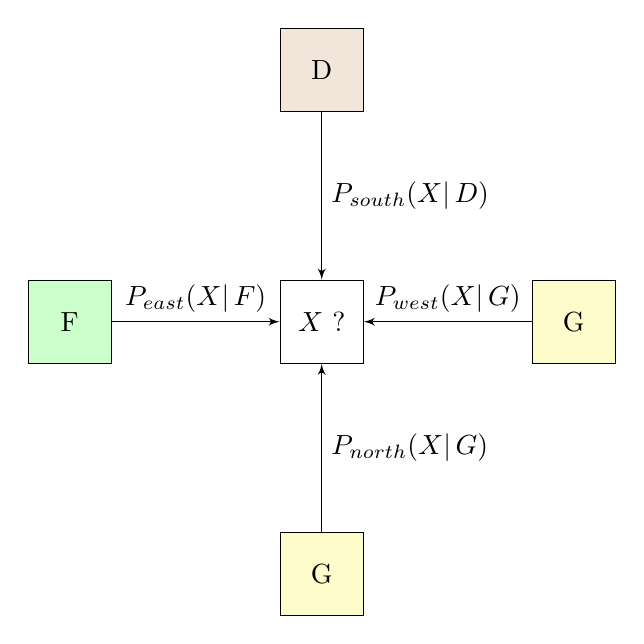
\begin{tikzpicture}[node distance = 3.2 cm, auto]
    \node[dcell](top){D};
    \node[ucell, below of=top](center){$X$~?};
    \node[fcell, left of=center](left){F};
    \node[gcell, right of=center](right){G};
    \node[gcell, below of=center](bottom){G};

    \path[line] (top)   -- node[right] {$P_{south}(X | \, D)$} (center);
    \path[line] (left)  -- node[above] {$P_{east}(X | \, F)$} (center);
    \path[line] (right) -- node[above] {$P_{west}(X | \, G)$} (center);
    \path[line] (bottom) -- node[right] {$P_{north}(X | \, G)$} (center);
\end{tikzpicture}
\end{center}

\caption{This situation includes a grass to the south and east, a dirt to the
    north and a forest to the west. It is similar to cell 2,19 in pallet town
    (when indexed from zero at the top left)}

\end{figure}

Suppose that the training set has the following characteristics:

\begin{table}[h]
\small
\begin{tabular}{ l | r r r r r r }
              & B      & D      & EDGE   & F      & G      & W \\ \hline
    north     & 0      & 0.1558 & 0.0519 & 0.0519 & 0.7403 & 0.0325\\
    east      & 0.0779 & 0.0974 & 0      & 0.1493 & 0.6428 & 0\\
    south     & 0      & 0.2403 & 0.0130 & 0.0065 & 0.7403 & 0\\
    west      & 0.0519 & 0.2273 & 0      & 0.0519 & 0.6428 & 0.0260\\
\end{tabular}
\caption{The probability of the class of neighbours in each direction for a
    grass cell from the map that we created entitled PalletTown} 
\end{table}


\subsection{Classifier Training}
\label{process:training}
\lipsum[1-2]


\section{Results}
\label{results}
\lipsum[1-2]


\subsection{Feature-Based Classifier}
\label{results:featurebased}
\lipsum[1-2]

\subsection{Gold Comparison Classifier}
\label{results:gold}
\lipsum[1-1]

\subsection{Proximity Classifier}
\label{results:proximity}
\lipsum[1-3]

\section{Conclusions}
\label{conclusions}
\lipsum[1-3]

\section{References}
\label{references}

%% The Appendices part is started with the command \appendix;
%% appendix sections are then done as normal sections
%% \appendix

%% \section{}
%% \label{}

%% References
%%
%% Following citation commands can be used in the body text:
%% Usage of \cite is as follows:
%%   \cite{key}          ==>>  [#]
%%   \cite[chap. 2]{key} ==>>  [#, chap. 2]
%%   \citet{key}         ==>>  Author [#]

%% References with bibTeX database:

\bibliographystyle{plain}
\bibliography{refs}

%% Authors are advised to submit their bibtex database files. They are
%% requested to list a bibtex style file in the manuscript if they do
%% not want to use model1-num-names.bst.

%% References without bibTeX database:

% \begin{thebibliography}{00}

%% \bibitem must have the following form:
%%   \bibitem{key}...
%%

% \bibitem{}

% \end{thebibliography}

\end{document}

